

\begin{frame}[fragile]{\shortt: Hipótesis}

\begin{center}
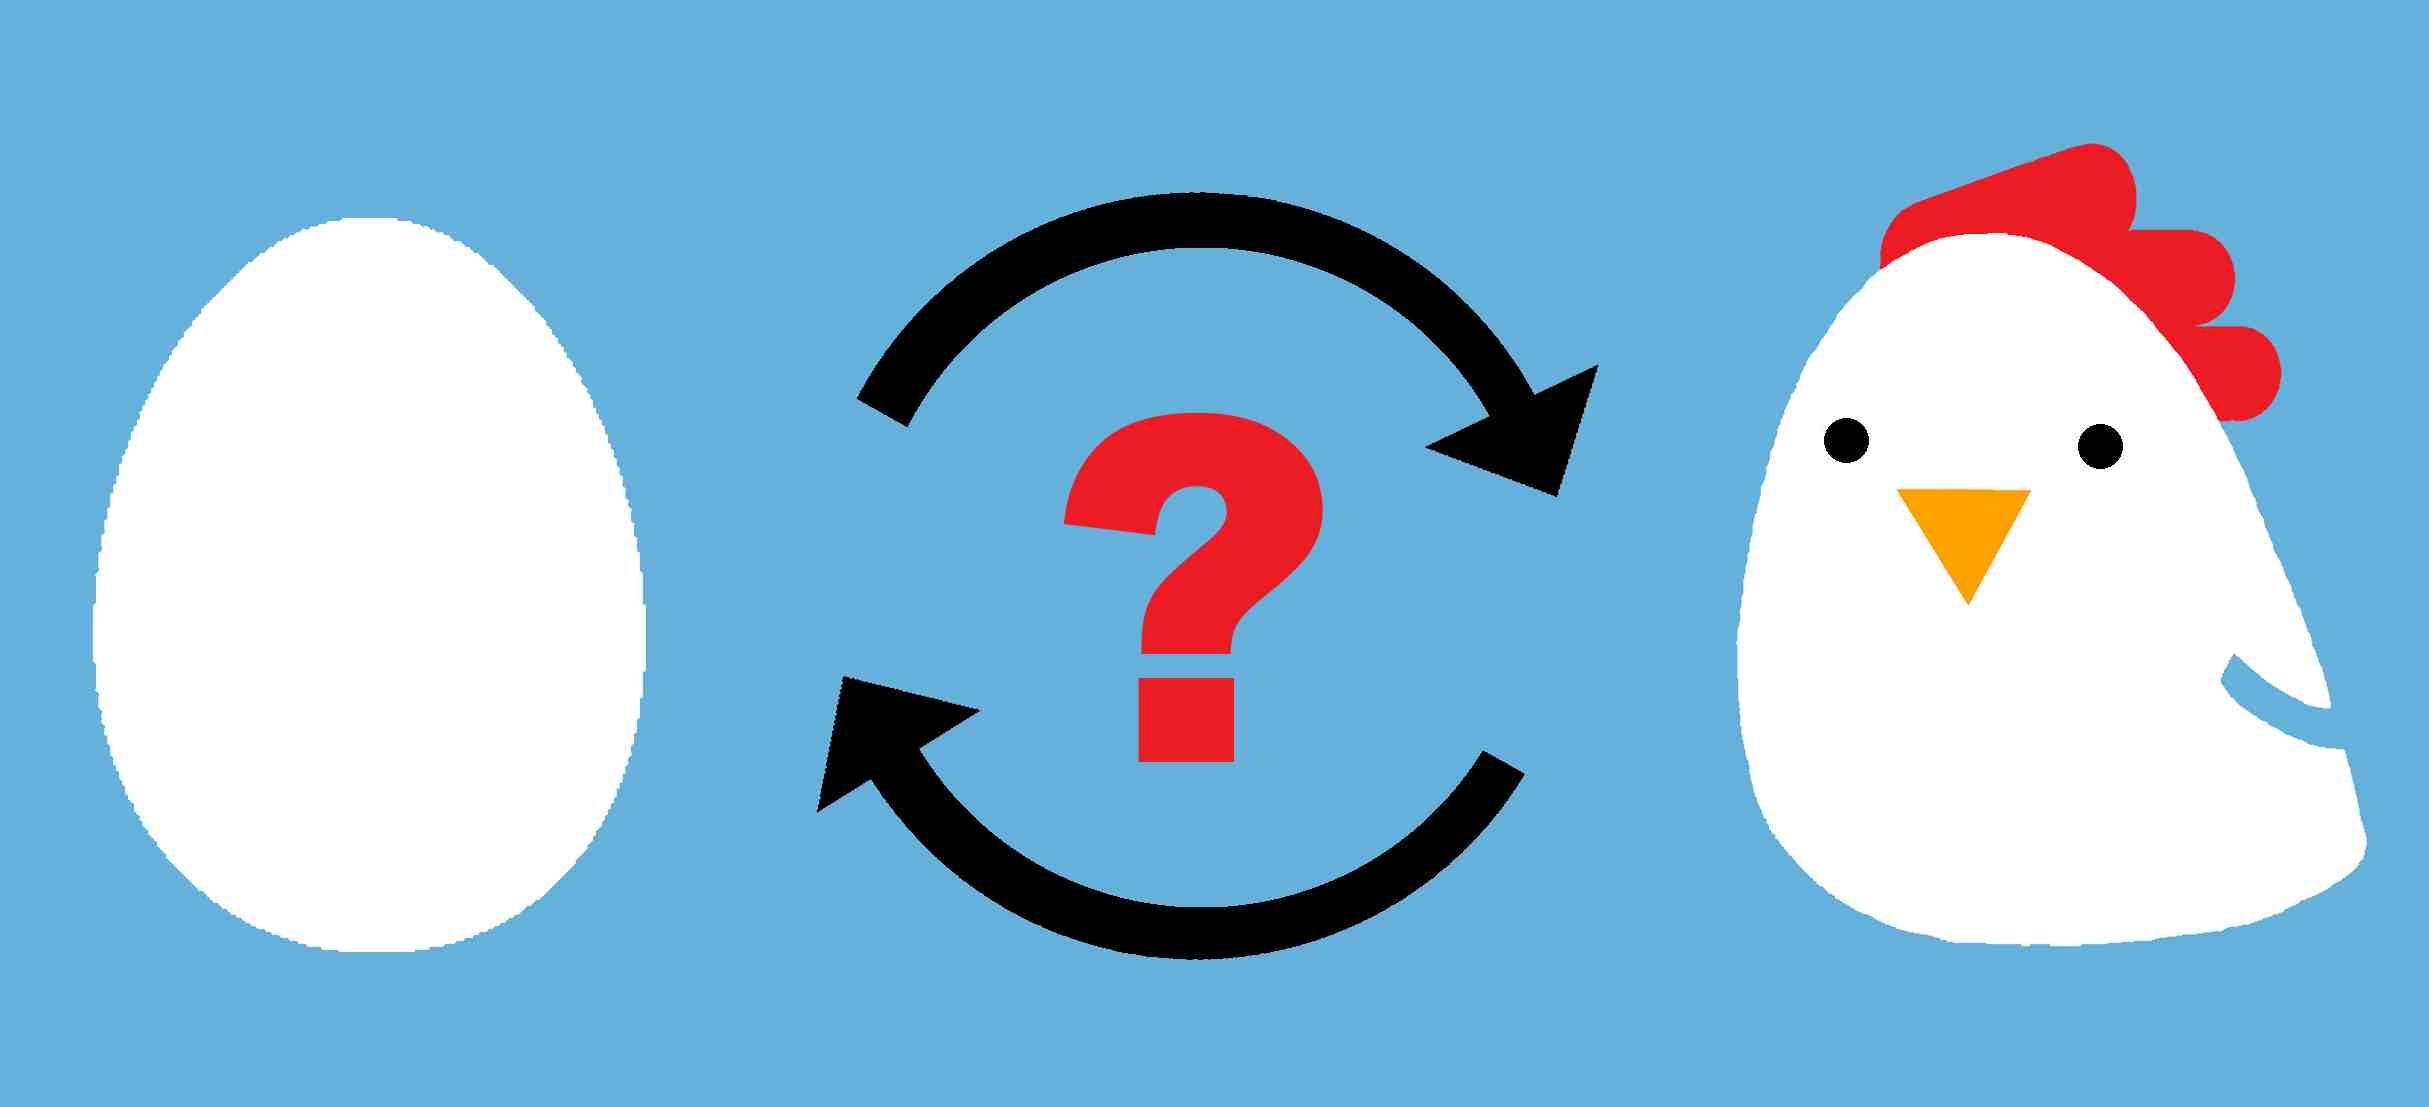
\includegraphics[scale=0.05]{images/gallina.jpg}
\end{center}
\begin{block}{Hipótesis}
\begin{itemize}
\item Los niños aprenden \alert{relaciones causales} velozmente y realizan inferencia causal de gran alcance a partir de observaciones. 

\item Los adultos pueden aprender estas relaciones, pero la experiencia hace que sus conclusiones estén sesgadas. 

\end{itemize}
\end{block}
\end{frame}

\begin{frame}[fragile]{\shortt: Trabajo Previo}


\begin{block}{Hasta el momento de publicación}

\begin{itemize}
\item No había estudios mostrando que los niños pueden aprender principios abstractos sobre la forma lógica de relaciones causales.
\item En consecuencia, tampoco comparaciones entre niños y adultos en su habilidad para realizarlo.
\item En el trabajo de \alert{Lucas and Griffiths (2010)} se encontró que los adultos pueden aprender \alert{sobrehipótesis} sobre relaciones causales y explicarlas en términos de un modelo Bayesiano jerárquico. Además, muestra que los adultos suelen estar predispuestos a relaciones disyuntivas y aprenden estas relaciones con mayor facilidad que las conjuntivas.
\end{itemize}    



\end{block}

\end{frame}

\begin{frame}[fragile]
\begin{block}{Sobre-hipótesis}
Se probaron dos principios causales:
\begin{itemize}
\item Forma disyuntiva: cada causa tiene una probabilidad independiente de causar un efecto.
\item Forma conjuntiva: causas independientes no pueden producir un efecto, pero el conjunto de ellas si.
\end{itemize}
\end{block}

\pause
Pero.. ¿Cuán buenos son los niños aprendiendo las sobrehipótesis?

\begin{exampleblock}{Pregunta}
¿Intuitivamente debería costarles más o menos que a los adultos? 
\end{exampleblock}

\pause
Varias investigaciones con enfoque Bayesiano indican que los niños tienen priors más débiles que le permiten adoptar nuevas hipótesis fácilmente y sin sesgos.


\end{frame}